\documentclass[UTF8,12pt]{ctexart}
\usepackage[a4paper,margin=24mm]{geometry}
\usepackage{amsmath,amssymb,bm,graphicx,adjustbox}
\newcommand{\fitmath}[1]{\begin{adjustbox}{max width=\linewidth}$\displaystyle #1$\end{adjustbox}}
\setlength{\parindent}{0pt}
\setlength{\parskip}{.7em}
\sloppy
\allowdisplaybreaks
\begin{document}
\section*{1989 年考研数学三 · 参考答案}
\subsection*{1989年真题参考答案}

\subsection*{（试卷IV）}

\subsection*{一、填空题}

（1）\(\displaystyle y=x+1\)。 （2）\(\displaystyle [-1,\allowbreak 1)\)。 （3）\(\displaystyle \lambda\) 为不等于1的任意常数。 （4）\(\displaystyle 1;\dfrac{\displaystyle 1}{\displaystyle 2}\)。 （5）\(\displaystyle \dfrac{\displaystyle 1}{\displaystyle 9}\)。


\subsection*{二、选择题}

（1）B。 （2）C。 （3）C。 （4）C。 （5）D。


\subsection*{三、计算题}

（1）\(\displaystyle e\)。 （2）\(\displaystyle \dfrac{\displaystyle \partial^2z}{\displaystyle \partial x\partial y}=\dfrac{\displaystyle \partial^2f}{\displaystyle \partial u^2}+(x+y)\dfrac{\displaystyle \partial^2f}{\displaystyle \partial u\partial v}+xy\dfrac{\displaystyle \partial^2f}{\displaystyle \partial v^2}+\dfrac{\displaystyle \partial f}{\displaystyle \partial v}\)。


（3）\(\displaystyle y(x)=C_1e^{-2x}+C_2e^{-3x}+e^{-x}\)，其中 \(\displaystyle C_1,\allowbreak C_2\) 为任意常数。


四、（1）收益函数 \(\displaystyle R(x)=10xe^{-x/2},\allowbreak \ 0\le x\le6\)，边际收益函数为 \(\displaystyle \dfrac{\displaystyle dR}{\displaystyle dx}=5(2-x)e^{-x/2}\)。（2）当产量为2时，收益最大，最大值为 \(\displaystyle 20e^{-1}\)，相应的价格为 \(\displaystyle 10e^{-1}\)。（3）如右图。


\begin{center}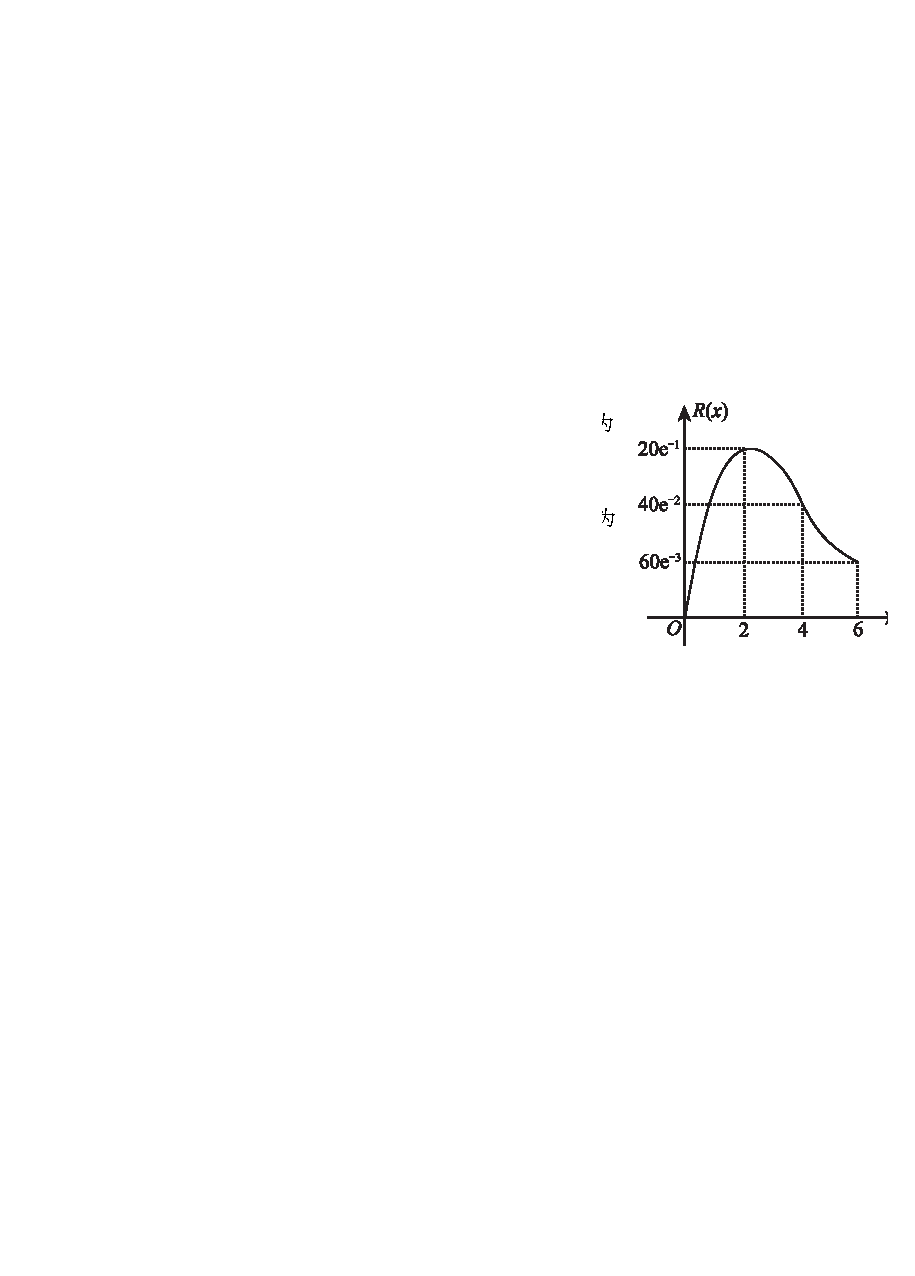
\includegraphics[width=.48\linewidth]{../assets/figures/page-064-10.pdf}\end{center}

五、（1）\(\displaystyle (1-e^{-1})^2\)。 （2）\(\displaystyle e^{-2}(1-e^{-1})^2\)。 （3）\(\displaystyle e^{-2n}(1-e^{-1})^2\)。 （4）\(\displaystyle \dfrac{\displaystyle e-1}{\displaystyle e+1}\)。


六、证明略（可利用积分中值定理）。


七、


\[\fitmath{\displaystyle X=\begin{pmatrix}3&-1\\2&0\\1&-1\end{pmatrix}.}\]


八、（1）当 \(\displaystyle t\ne5\) 时，向量组 \(\displaystyle \boldsymbol\alpha_1,\allowbreak \boldsymbol\alpha_2,\allowbreak \boldsymbol\alpha_3\) 线性无关。（2）当 \(\displaystyle t=5\) 时，向量组线性相关。（3）当向量组线性相关时，\(\displaystyle \boldsymbol\alpha_3=-\boldsymbol\alpha_1+2\boldsymbol\alpha_2\)。


九、（1）\(\displaystyle 1,\allowbreak 1,\allowbreak -5\)。 （2）\(\displaystyle 2,\allowbreak 2,\allowbreak \dfrac{\displaystyle 4}{\displaystyle 5}\)。


十、（1）\(\displaystyle \dfrac{\displaystyle 1}{\displaystyle 2}\)。 （2）\(\displaystyle 1\)。


十一、\(\displaystyle \dfrac{\displaystyle 20}{\displaystyle 27}\)。


\subsection*{（试卷V）}

\subsection*{一、填空题}

（1）【同试卷IV 第一、（1）题】 （2）\(\displaystyle b\)。 （3）\(\displaystyle x^4\)。 （4）\(\displaystyle 46\)。 （5）【同试卷IV 第一、（4）题】


\subsection*{（试卷V）参考答案续}

\subsection*{二、选择题}

（1）【同试卷IV 第二、（1）题】 （2）【同试卷IV 第二、（2）题】 （3）【同试卷IV 第二、（3）题】 （4）B。 （5）【同试卷IV 第二、（5）题】


\subsection*{三、计算题}

（1）\(\displaystyle e\)。 （2）\(\displaystyle dz=\dfrac{\displaystyle z\ln a}{\displaystyle \sqrt{x^2-y^2}}(x\,dx-y\,dy)\)。 （3）\(\displaystyle (1-\dfrac{\displaystyle 1}{\displaystyle x})\ln(1-x)+C\)，其中 \(\displaystyle C\) 为任意常数。 （4）\(\displaystyle \dfrac{\displaystyle \pi}{\displaystyle 2}(\ln2-\dfrac{\displaystyle 1}{\displaystyle 2})\)。


四、（1）利润函数 \(\displaystyle L=R-C=18x-3x^2-4x^3\)。（2）边际收入函数 \(\displaystyle MR=\dfrac{\displaystyle dR}{\displaystyle dx}=26-4x-12x^2\)。（3）边际成本函数 \(\displaystyle MC=\dfrac{\displaystyle dC}{\displaystyle dx}=8+2x\)。（4）当产量为1时，利润最大，最大利润为11。


五、函数的单增区间为 \(\displaystyle (0,\allowbreak 1)\)，单减区间为 \(\displaystyle (-\infty,\allowbreak 0),\allowbreak (1,\allowbreak +\infty)\)。函数在点 \(\displaystyle x=0\) 处取得极小值，极小值为0。函数图形在 \(\displaystyle (-\infty,\allowbreak -\dfrac{\displaystyle 1}{\displaystyle 2})\) 上是凸的，在 \(\displaystyle (-\dfrac{\displaystyle 1}{\displaystyle 2},\allowbreak 1)\) 和 \(\displaystyle (1,\allowbreak +\infty)\) 上是凹的，\(\displaystyle (-\dfrac{\displaystyle 1}{\displaystyle 2},\allowbreak \dfrac{\displaystyle 2}{\displaystyle 9})\) 是曲线的拐点。\(\displaystyle y=2\) 为图形的水平渐近线，\(\displaystyle x=1\) 为图形的铅直渐近线。


\begin{center}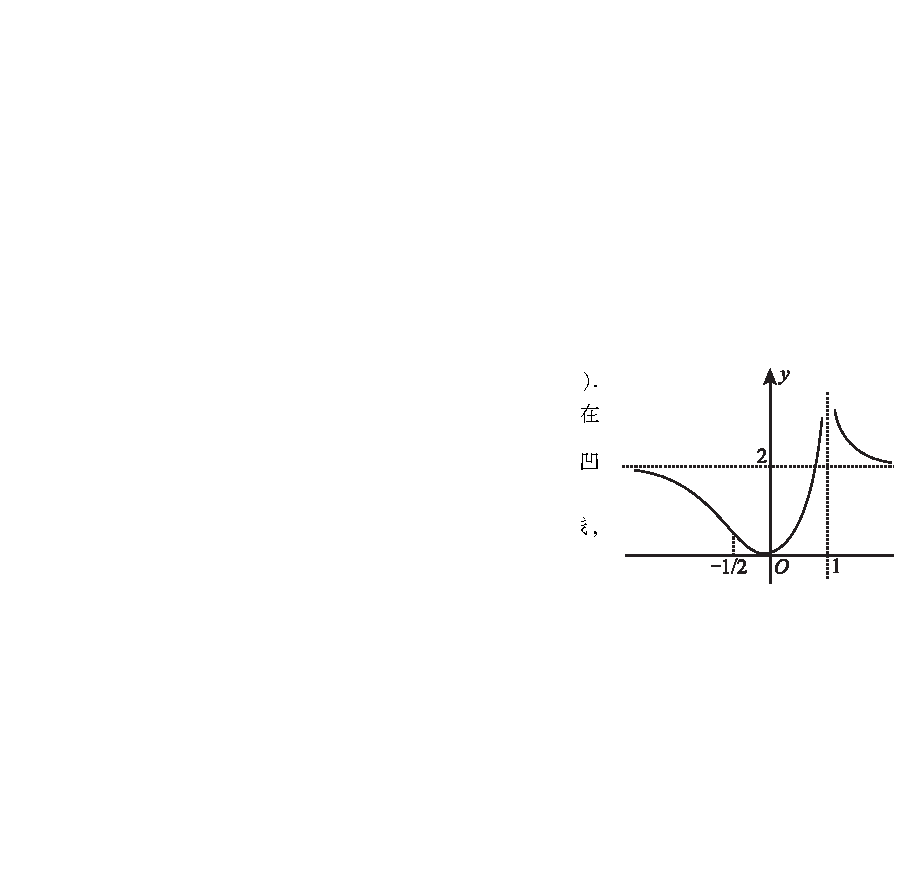
\includegraphics[width=.48\linewidth]{../assets/figures/page-065-07.pdf}\end{center}

六、【同试卷IV 第七题】


七、当 \(\displaystyle t\ne1\) 时，向量组 \(\displaystyle \boldsymbol\alpha_1,\allowbreak \boldsymbol\alpha_2,\allowbreak \boldsymbol\alpha_3\) 线性无关；当 \(\displaystyle t=1\) 时，向量组线性相关。


八、【同试卷IV 第九题】


九、（1）


\[\fitmath{\displaystyle \begin{array}{c|ccc}x&0&1&2\\\hline P\{X=x\}&0.25&0.45&0.30\end{array}}\]


（2）


\[\fitmath{\displaystyle \begin{array}{c|cccc}s&0&1&2&3\\\hline P\{X+Y=s\}&0.10&0.40&0.35&0.15\end{array}}\]


（3）\(\displaystyle 0.25\)。


十、\(\displaystyle 1-e^{-1}\)。

\end{document}
